\documentclass[12pt, a4paper]{article}
\usepackage[utf8]{inputenc}
\usepackage{listings}
\usepackage[IL2]{fontenc}
\usepackage[czech]{babel}
\usepackage{graphicx}
\usepackage{mathtools}
\usepackage{amsmath}
\usepackage{flafter} 
\usepackage[pdfborder={0 0 0}]{hyperref}

\title{\textbf{Dokumentace semestrální práce} \\KIV/PT}
\author{Vojtěch Danišík}
\begin{document}

\begin{titlepage} 
	\newcommand{\HRule}{\rule{\linewidth}{0.5mm}} 
	\begin{center}
	
\includegraphics[width=6cm]{img/logo}\\
	\end{center}
	\textsc{\LARGE Západočeská univerzita v Plzni}\\[1.5cm] 	
	\textsc{\Large Úvod do počítačových sítí}\\[0.5cm] 
	\textsc{\large KIV/UPS}\\[0.5cm] 
	\HRule\\[0.4cm]
	{\LARGE\bfseries Dokumentace semestrální práce - Dáma}\\[0.4cm] 
	\HRule\\[1.5cm]

	\begin{minipage}{0.4\textwidth}
		\begin{flushleft}
			\large
			Vojtěch \textsc{Danišík}\newline
			A16B0019P\newline
			danisik@students.zcu.cz
		\end{flushleft}
	\end{minipage}
	\vfill\vfill\vfill
	\begin{flushright}
	{\large\today}
	\end{flushright}
	\vfill 
\end{titlepage}
\newpage
\tableofcontents
\newpage
\section{Zadání}
Vytvořte program realizující vybranou hru. Vytvořte  server, který bude obsluhovat více hráčů i her současně a bude schopen uložit stav
hry. Klient bude po opětovném přihlášení pokračovat tam, kde přestal. Přenosový protokol je TCP. Jazyk použitý pro server: C. 
Jazyk použitý pro klienta: Java. Vybraná hra je \textbf{Dáma} .
\begin {figure}[h]
\centering
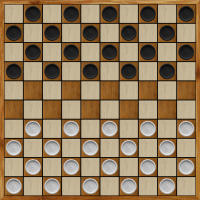
\includegraphics[width=6cm]{img/draughts_example}
\caption{Hrací pole dámy}
\label{fig:draughts_example}
\end {figure}

%% SECTION %%
\section{Programátorská dokumentace}
\label{Programátorská dokumentace}
%% SUBSECTION %%
\subsection{Server}
\label{Server}
Server je naprogramován v jazyce \textbf{C}.
%% SUBSUBSECTION %%
\subsubsection{Datové struktury}
\label{Server_Datové_struktury}
Server používá pro svůj běh tyto datové struktury:
\begin{itemize}
\item STATES (enum) - Konstantní proměnné použité jako stavy pro jednotlivé hráče, ve kterých se mohou nacházet
\item client - Struktura pro uložení hráče
	\begin{itemize}
	\item (char*) name - Jméno hráče zvolené při přihlášení
	\item (int) socket\_ID - Socket ID hráče získané při připojení na server
	\item (char*) color - Barva hráče, kterou mu server přiřadí při spuštění hry
	\item (STATES) state - Stav, ve kterém se hráč nachází
	\end{itemize}
\item clients - Struktura pro uložení všech klientů do pole
	\begin{itemize}
	\item (int) clients\_count - Počet přihlášených hráčů
	\item (client**) clients - Pole klientů
	\end{itemize}	 
\item piece - Hrací figurka
	\begin{itemize}
	\item (char*) color - Barva figurky (black/white)
	\item (char*) type - Typ figurky (man/king)
	\end{itemize}	 
\item field - Políčko hrací plochy
	\begin{itemize}
	\item (int) row - Řádek políčka na hrací ploše
	\item (int) col - Sloupec políčka na hrací ploše
	\item (char*) color - Barva políčka
	\item (piece*) piece - Figurka na políčku (políčko může obsahovat figurku)
	\end{itemize}	 
\item fields - Struktura pro uložení všech políček
	\begin{itemize}
	\item (int) size - Velikost hrací plochy
	\item (field***) all\_fields - Pole všech políček na hrací ploše
	\item (int) count\_pieces - Počet políček na hrací ploše 
	\end{itemize}	 
\item wanna\_play - Struktura pro zjištění, kteří hráči chtějí hrát hru
	\begin{itemize}
	\item (int) size - Počet hráčů, kteří chtějí hrát hru
	\item (int*) socket\_IDs - Pole ID socketů hráčů
	\end{itemize}	 
\item game - Struktura reprezentující hru
	\begin{itemize}
	\item (char*) name\_1 - Jméno prvního hráče
	\item (char*) name\_2 - Jméno druhého hráče
	\item (char*) now\_playing - Aktuálně hrající hráč
	\item (int) game\_ID - ID hry
	\item (fields*) fields - Hrací plocha
	\end{itemize}	 
\item games - Struktura pro uložení všech her
	\begin{itemize}
	\item (int) games\_count - Počet rozehraných her
	\item (game**) games - Pole všech rozehraných her
	\end{itemize}	 
\item log\_info - Struktura pro uložení logovacích informací
	\begin{itemize}
	\item (int) count\_bytes - Počet přenesených bytů
	\item (int) count\_messages - Počet přenesených zpráv
	\item (int) count\_connections- Počet připojení na server
	\item (int) count\_bad\_transmissions - Počet špatných přenosů
	\item (int) server\_running\_minutes - Čas běhu serveru (v minutách)
	\end{itemize}	 
\end{itemize}
%% SUBSUBSECTION %%
\subsubsection{Formáty zpráv}
\label{Server_Formáty_zpráv}
\begin{table}[!hbt]
\centering
\begin{tabular}{|l|l|} 
\hline
\textbf{Předpis} & \textbf{Význam}                            \\ 
\hline
\textit{login\_ok;} & Uživatel přihlášen                 \\ 
\hline
\textit{login\_false;error\_ID;}  & Uživatel nepřihlášen + číslo erroru                     \\ 
\hline
\textit{start\_game;player\_color;game\_ID;}  & Nová hra vytvořena a startnuta                     \\
\hline
\begin{tabular}[c]{@{}l@{}}
\textit{correct\_move;move\_type;cp\_row;}\\\textit{cp\_col;dp\_row;dp\_col;}\end{tabular}  & Správný tah                     \\ 
\hline
\textit{end\_move;}  & Konec tahu aktuálního hráče                     \\
\hline
\textit{wrong\_move;error\_ID;}  & Špatný tah                     \\ 
\hline
\textit{update\_game\_ID;game\_ID;}  & Update game ID                     \\ 
\hline
\textit{play\_next\_player;}  & Hraje druhý hráč                     \\ 
\hline
\textit{end\_game;player\_state;}  & Korektní konec hry (žádný error)                     \\ 
\hline
\textit{end\_game\_left;error\_ID;}  & Nekorektní konec hry, oponent ukončil hru                     \\ 
\hline
\textit{end\_game\_timeout;error\_ID;}  & Nekorektní konec hry, oponent se nepřipojil                     \\ 
\hline
\textit{opponent\_connection\_lost;}  & Oponent ztratil připojení k internetu                     \\ 
\hline
\textit{connection\_restored;}  & Oponent se vrátil do hry                     \\ 
\hline
\textit{promote;dp\_row;dp\_col;}  & Vylepšení figurky muže na krále                     \\ 
\hline
\begin{tabular}[c]{@{}l@{}}
\textit{board;name;player\_color;game\_ID;}\\\textit{count\_pieces;who\_play;piece\_x;piece\_y;}\\\textit{piece\_color;piece\_type;....;}  \end{tabular}& Aktuální hrací plocha hry                    \\
\hline
\end{tabular}
\end{table}
\newpage
\large{\textbf{Legenda}}
\newline\textit{error\_ID} - ID erroru, podle kterého se vypíše určitá hláška u klienta
\newline\textit{player\_color} - Barva hráče, za kterou bude hrát
\newline\textit{game\_ID} -  ID hry
\newline\textit{move\_type} - Typ pohybu (2 - klasický pohyb, 3 - pohyb s přeskokem oponenta)
\newline\textit{cp\_row} - Řádek figurky, ze které skáču
\newline\textit{cp\_col} - Sloupec figurky, ze které skáču
\newline\textit{dp\_row} - Řádek figurky, na kterou skáču
\newline\textit{dp\_col} - Sloupec figurky, na kterou skáču
\newline\textit{player\_state} - Hráčův stav po konci hry (win - výhra, draw - remíza, lose - prohra)
\newline\textit{count\_pieces} - Aktuální počet figurek ve hře
\newline\textit{who\_play} -  Kdo je momentálně na tahu ve hře
\newline\textit{piece\_x} - Řádek figurky 
\newline\textit{piece\_y} - Sloupec figurky
\newline\textit{piece\_color} -  Barva figurky (white - bílá, black - černá)
\newline\textit{piece\_type} - Typ figurky (man - muž, king - král)
\newline\textit{....} - Opakování parametrů od piece\_x do piece\_type
%% SUBSECTION %%
\subsection{Klient}
\label{Klient}
Klient je naprogramován v jazyce \textbf{Java}.
%% SUBSUBSECTION %%
\subsubsection{Datové struktury}
\label{Klient_Datové_struktury}
Klient obsahuje tyto balíčky s třídami:
\begin{itemize}
\item connection - Třídy pracující s připojením k serveru, čtením a odesíláním zpráv. Je zde klient reprezentující hráče, čtecí vlákno, které na základě přijmuté zprávy vykoná činnost (zobrazí nové okno).
\item constants - Konstanty aplikace (Velikosti okna, zobrazované texty, názvy komponent, ...)
\item enums - Výčtové typy (Barvy použité v aplikaci - pro políčka, zvýraznění textu, ...; Posílané a přijímané zprávy;Typy figurek; ID chybových hlášení a jejich převod na text)
\item field - Třídy generující políčka do hry
\item main -  Hlavní spouštěcí třída
\item messages - Třídy reprezentující přijímané a odesílané zprávy na server
\item piece - Třídy reprezentující figurky
\item windows - Hlavní vykreslovací třída 
\item client - Struktura pro uložení hráče
\end{itemize}
%% SUBSUBSECTION %%
\subsubsection{Formáty zpráv}      
\label{Klient_Formáty_zpráv}  
\begin{table}[!hbt]
\centering
\begin{tabular}{|l|l|} 
\hline
\textbf{Předpis} & \textbf{Význam}                            \\ 
\hline
\textit{login;name;} & Uživatel se chce přihlásit                 \\ 
\hline
\textit{play;}  & Uživatel chce hrát hru                     \\ 
\hline
\begin{tabular}[c]{@{}l@{}}
\textit{client\_move;game\_ID;cp\_row;cp\_col;}\\\textit{dp\_row;dp\_col;piece\_color;piece\_type;}
\end{tabular} & Uživatel chce pohnout figurkou             \\ 
\hline
\textit{new\_game\_no;} & Uživatel nechce hrát novou hru  \\
\hline
\end{tabular}
\end{table}
\large{\textbf{Legenda}}
\newline\textit{name} - Jméno hráče
\newline\textit{game\_ID} -  ID hry
\newline\textit{cp\_row} - Řádek figurky, ze které skáču
\newline\textit{cp\_col} - Sloupec figurky, ze které skáču
\newline\textit{dp\_row} - Řádek figurky, na kterou skáču
\newline\textit{dp\_col} - Sloupec figurky, na kterou skáču
\newline\textit{piece\_color} -  Barva figurky (white - bílá, black - černá)
\newline\textit{piece\_type} - Typ figurky (man - muž, king - král)
%% SUBSECTION %%
\subsection{Implementace}
\label{Implementace}
%% SUBSUBSECTION %%
\subsubsection{Start serveru}
\label{Start_serveru}
Server se po startu snaží obsadit port zadaný při startu (pokud není zadán, použije se defaultní port 10000), pokud se mu to podaří, vypíše server do konzole \textit{Bind OK}
\newline
Přijde-li příchozí spojení (socket), server vytvoří sadu deskriptorů pomocí metody \textit{select()} a začne jednomu z tří desktriptorů naslouchat (jeden slouží pro read, druhý pro write, třetí pro chybové hlášení).
%% SUBSUBSECTION %%
\subsubsection{Zpracování příchozích zpráv}
\label{Server_Zpracování_příchozích_zpráv}
Každý klient má svůj vlastní desktriptor, který mu naslouchá a stará se o příjem. Po přijmutí zprávy jej rozparsuje a vyhodnotí. Povoleny jsou jen zprávy se správným formátem, viz \ref{Server_Formáty_zpráv}
%% SUBSUBSECTION %%
\subsubsection{Vytvoření nové hry}
\label{Vytvoření_nové_hry}
Klient po přihlášení na server má možnost se připojit do fronty hráčů, kteří chtějí hrát hru. Pokud jsou ve frontě alespoň 2 hráči, server vybere posledního hráče, který chce hrát a náhodně z fronty druhého hráče a spojí je do jedné hry. Každému klientovy bude náhodně přiřazena barva a odeslána zpráva s jejich barvou a ID hrou.
%% SUBSUBSECTION %%
\subsubsection{Připojení do rozehrané hry}
\label{Připojení_do_rozehrané_hry}
Pokud klient vypadne, přejde do stavu \textit{disconnect} a spustí se timeout, který je nastavený na \textbf{10 minut}. Pokud se do té doby klient pod stejným jménem přihlásí, bude vpuštěn do rozehrané hry, ve které byl před tím, než ztratil spojení. Server tomuto klientovy odešle ID hry, počet figurek a jejich pozice, barvu a typ, aby se klient mohl ihned zapojit do hry.
%% SUBSUBSECTION %%
\subsubsection{Konec hry}
\label{Konec_hry}
Když hra skončí korektně (jeden hráč sebere všechny figurky tomu druhému), tak je na serveru vyhodnoceno kdo vyhrál/prohrál nebo zda je remíza a jednotlivé výsledky jsou rozeslány hráčům. Ti mají možnost hrát znovu či nikoliv. Pokud by se jeden z hráčů během hry odpojil ze hry tím, že ukončí klienta i přes to, že mu spojení se serverem funguje, je hra ukončena, druhý hráč informován o tom, že oponent odešel ze hry a automaticky vyhrává.
%% SECTION %%
\section{Uživatelská dokumentace}
\label{Uživatelská_dokumentace}
%% SUBSECTION %%
\subsection{Překlad}
\label{Překlad}
Přeložení zdrojových souborů se provádí zadáním příkazu \textit{make} v terminálu v kořenovém adresáři staženého souboru. Zdrojové soubory pro klienta najdeme ve složce \textbf{\/java\_src\/} a pro server ve složce \textbf{\/c\_src\/}.
 %% SUBSECTION %%
\subsection{Spuštění serveru}
\label{Spuštění_serveru}
Server se spouští pomocí příkazu \textit{./server -port [port\_ID]}, kde \textit{port\_ID} je číslo portu v rozsahu 1024 - 65535, na kterém bude server naslouchat.
 %% SUBSECTION %%
\subsection{Spuštění klienta}
\label{Spuštění_klienta}
Klient se spouští pomocí příkazu \textit{java -jar client.jar -address [address] -port [port\_ID]}, kde \textit{address} je IPv4 adresa serveru a \textit{port\_ID} je číslo portu v rozsahu 1024 - 65535, na kterém bude klient naslouchat.
\newline
Po spuštění .jar souboru se otevře přihlašovací okno, kde se zadá jméno, pod kterým bude uživatel hrát. Pokud je toto jméno volné, server vás přihlásí. Pokud bude zabrané, server pošle chybové hlášení.
\begin {figure}[h]
\centering
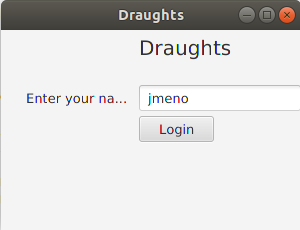
\includegraphics[width=6cm]{img/login}
\caption{Přihlašování}
\label{fig:login}
\end {figure}
\newline
Po přihlášení se dostaneme do lobby okna, ve kterém po kliknutí na tlačítko \textit{Play} budete přidáni do fronty pro hráče čekající na hru. Pokud ve frontě budou alespoň 2 hráči, budete přiřazeni do hry.
\begin {figure}[h]
\centering
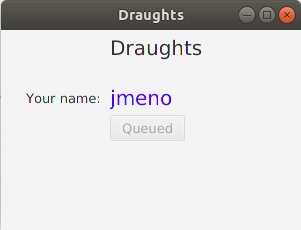
\includegraphics[width=6cm]{img/lobby}
\caption{Lobby}
\label{fig:lobby}
\end {figure}
\newline
Po úspěšném přiřazení do hry vám bude přiřazena náhodně serverem barva, za kterou budete hrát. Tuto barvu uvidíte v pravém horním rohu (bílá/černá). Hraní dámy funguje následovně: 
\begin{itemize}
\item Kliknutí na svojí figurku a posunout jí kliknutím na novou pozici vzhledem k pravidlům dámy. Po každém kliknutí lze vidět pozici políčka, na které jste kliknuli a typ a barva figurky, pokud se nachází na políčku.
\item Pokud je krok nevalidní, server pošle chybovou hlášku, která se zobrazí právě hrajícímu klientovy s textem, jaký nevalidní krok klient provedl. Pokud je krok validní, pouze se v pravé části okna zobrazí \textit{Now playing: Opponent}.
\end{itemize}
\begin {figure}[h]
\centering
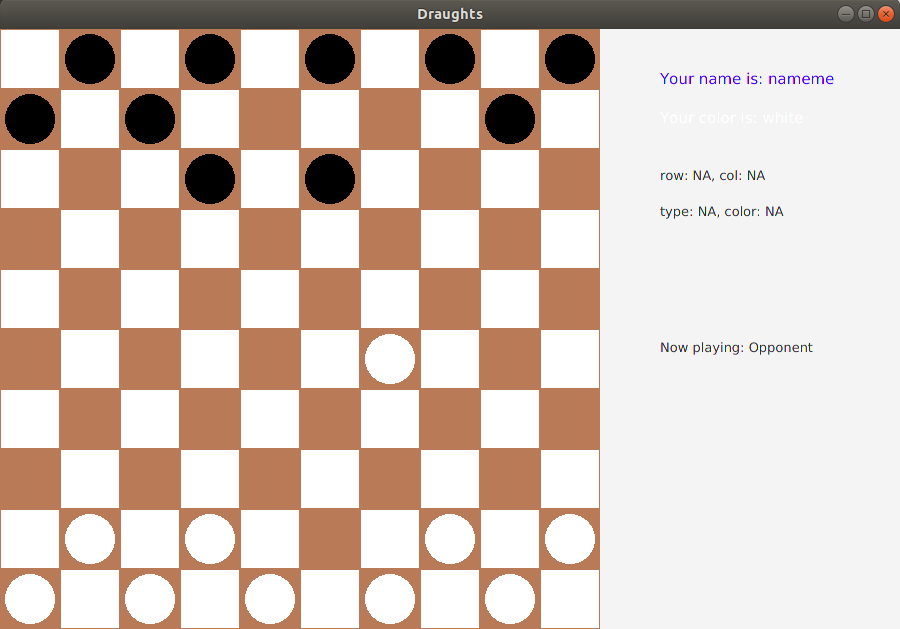
\includegraphics[width=10cm]{img/ingame}
\caption{Hra dáma}
\label{fig:hra}
\end {figure}
\section{Závěr}
Práce splňuje zadání, server umí odbavit požadavky několika klientů najednou a zároveň je natolik stabilní, aby jej výpadek nebo chyba jednoho z klientů neukončila chybou. Klient lze spustit na systému Linux i Windows (testováno na Windows 10), server byl testován na systému Linux – konkrétně na distribuci Ubuntu 18.04.1 LTS.
\end{document}